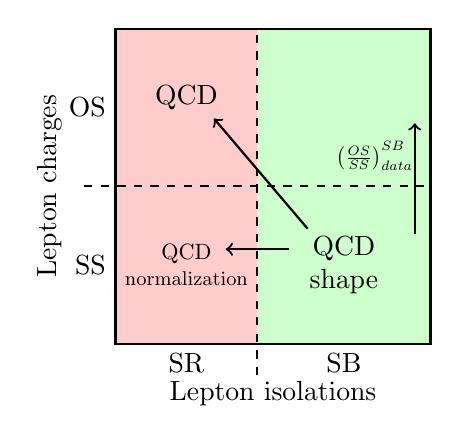
\begin{tikzpicture}[scale=4]
  
    \def\mx{0.45} %middle
    
    % boxes
    \fill [red!20!white] % SR
      (0,0) rectangle (\mx,1);
    \fill [green!20!white] % SB
      (\mx,0) rectangle (1,1);
    \draw[thick]
      (0,0) rectangle (1,1);
    
    % dashed lines
    \draw[dashed,thick]
      (\mx,-0.1) -- (\mx,1);
    \draw[dashed,thick]
      (-0.1,0.5) -- (1,0.5);
    
    % labels
    \draw
      (0,0.75) node[anchor=east]  {OS}
      (0,0.25) node[anchor=east]  {SS}
      (\mx/2,0) node[anchor=north] {SR}
      (0.5+\mx/2,0) node[anchor=north] {SB}
      (0,0.50) node[rotate=90,above=16pt] {Lepton charges}
      (0.50,0) node[below=10pt] {Lepton isolations};
    \draw
      (\mx/2,0.78) node {QCD}
      (0.5+\mx/2,0.25) node[align=center] {QCD\\shape} %{$\text{QCD}^\text{SS,SB}_\text{data}$};
      (\mx/2,0.25) node[align=center,scale=0.80] {QCD\\\small normalization};
    
    % arrows
    \draw[->,thick] % SR: SS -> OS
      (\mx+0.1,0.30) -- (\mx-0.1,0.30);
      %node[midway,above=8pt,right=-2pt,scale=0.70]{};
    \draw[->,thick] % SB: SS -> OS
      (0.95,0.35) -- (0.95,0.7)
      node[midway,above=8pt,left=-2pt,scale=0.70]{$\left(\frac{\text{OS}}{\text{SS}}\right)^\text{\tiny SB}_\text{\tiny data}$};
    
    \begin{scope}[shift={(\mx+0.02,0.54)},scale=0.35]
      \draw[->,thick]
        (0.40,-0.5) -- (-0.45,0.5);
        %node[midway,above=5pt,right=0pt,scale=0.8]{ $F^{\tiny \text{e}\mu}_\text{\tiny sim}$};
    \end{scope}
    
  \end{tikzpicture}